\section{Assignment 2}

\subsection{Implement in MATLAB the trapezoidal trajectory taking into account the different constraints.}

The general expression for a trapezoidal velocity profile is:

\begin{equation*}
q(t)=\begin{cases}
q_i+\dot q_i(t-t_i)+\frac{\dot q_c-\dot q_i}{2t_a}(t-t_i)^2 & t_i\leq t\leq t_a+t_i\\
q_i+\dot q_i\frac{t_a}{2}+\dot q_c(t-t_i-\frac{t_a}{2})^2 & t_a+t_i\leq t\leq t_f-t_d\\
q_f-\dot q_f(t_f-t)-\frac{\dot q_c-\dot q_f}{2t_d}(t_f-t)^2 & t_f-t_d\leq t\leq t_f
\end{cases}
\end{equation*}

If the initial and final velocities are null, then $t_a=t_d=t_c$.

If $\dot q_i=\dot q_f=0$ then the possible constraints are:
\begin{itemize}
\item $t_c$:
\begin{equation*}
\ddot q_c = \frac{q_f-q_i}{t_ct_f-t_c^2}\;\;\;\;\dot q_c=\ddot q_ct_c
\end{equation*}
\item $\ddot q_c$:
\begin{equation*}
t_c=\frac{t_f}{2}-\frac{1}{2}\sqrt{\frac{t_f^2\ddot q_c-4(q_f-q_i)}{\ddot q_c}}\;\;\;\;\dot q_c=\ddot q_ct_c
\end{equation*}
\item $\dot q_c$:
\begin{equation*}
t_c=\frac{q_i-q_f+\dot q_ct_f}{\dot q_c}\;\;\;\;\ddot q_c = \frac{\dot q_c^2}{q_i-q_f+\dot q_ct_f}
\end{equation*}
\item $\ddot q_c,\dot q_c$:
\begin{equation*}
t_c=\frac{\dot q_c}{\ddot q_c}\;\;\;\;t_f=\frac{\dot q_c^2+\ddot q_c(q_f-q_i)}{\dot q_c\ddot q_c}
\end{equation*}
\end{itemize}

In all cases the feasibility condition is that $2t_c\leq t_f-t_i$.

If $\dot q_i,\dot q_f\neq 0$ the possible constraints are:

\begin{itemize}
\item $\ddot q_{c,max}$:
\begin{equation*}
\dot q_c = \frac{1}{2}(\dot q_i+\dot q_f+\ddot q_{c,max}\Delta T+\sqrt{\ddot q_{c,max}^2\Delta T^2-4\ddot q_{c,max}\Delta q+2\ddot q_{c,max}(\dot q_i+\dot q_f)\Delta T-(\dot q_i-\dot q_f)^2}\;\;\;\;\;t_a=\frac{\dot q_c-\dot q_i}{\ddot q_{c,max}}\;t_d=\frac{\dot q_c-\dot q_f}{\ddot q_{c,max}}
\end{equation*}

The trajectory is feasible when the argument of the square root is positive, and when the maximum acceleration satisfies:

\begin{equation*}
\ddot q_{c,max}\Delta q>\frac{\abs{\dot q_i^2-\dot q_f^2}}{2}\;\;\;\ddot q_{c,max}\geq\ddot q_{c,lim}=\frac{2\Delta q-(\dot q_i-\dot q_f)\Delta T+\sqrt{4\Delta q^2-4\Delta q(\dot q_i+\dot q_f)\Delta T+2(\dot q_i^2+\dot q_f^2)\Delta T^2}}{\Delta T^2}
\end{equation*}

when $\ddot q_{c,max}=\ddot q_{c,lim}$ there is no constant velocity phase.
\item $\ddot q_{max},\dot q_{max}$:
First we compute the condition:
\begin{equation*}
\ddot q_{c,max}\Delta q\gtreqless\dot q_{c,max}^2-\frac{\dot q_i^2+\dot q_f^2}{2}
\end{equation*}

If the above is $>$ then:

\begin{equation*}
\dot q_c=\dot q_{c,max}\;\;\;t_a=\frac{\dot q_{c,max}-\dot q_i}{\ddot q_{c,max}}\;\;\;t_d=\frac{\dot q_{c,max}-\dot q_f}{\ddot q_{c,max}}\;\;\;\Delta T=\frac{\Delta q\ddot q_{c,max}+\dot q_{c,max}^2}{\ddot q_{c,max}\dot q_{c,max}}
\end{equation*}

If the above is $\leq$ then:
\begin{equation*}
\dot q_c=\dot q_{c,lim}=\sqrt{\ddot q_{c,max}\Delta q+\frac{\dot q_i^2+\dot q_f^2}{2}}<\dot q_{c,max}\;\;\;t_a=\frac{\dot q_{c,lim}-\dot q_i}{\ddot q_{c,max}}\;\;\;t_d=\frac{\dot q_{c,lim}-\dot q_f}{\ddot q_{c,max}}
\end{equation*}
\end{itemize}

\begin{figure}
\begin{minipage}{0.333\textwidth}
\centering
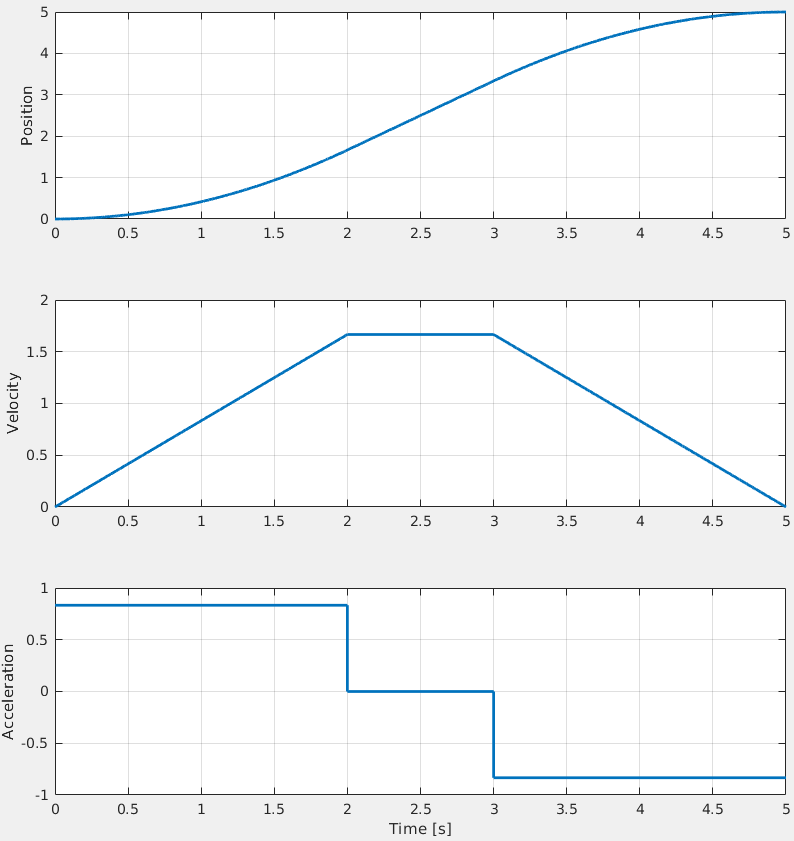
\includegraphics[keepaspectratio,width=\textwidth]{trap_1}
\caption{$t_c=2s$}
\label{fig:trap_1}
\end{minipage}
\begin{minipage}{0.333\textwidth}
\centering
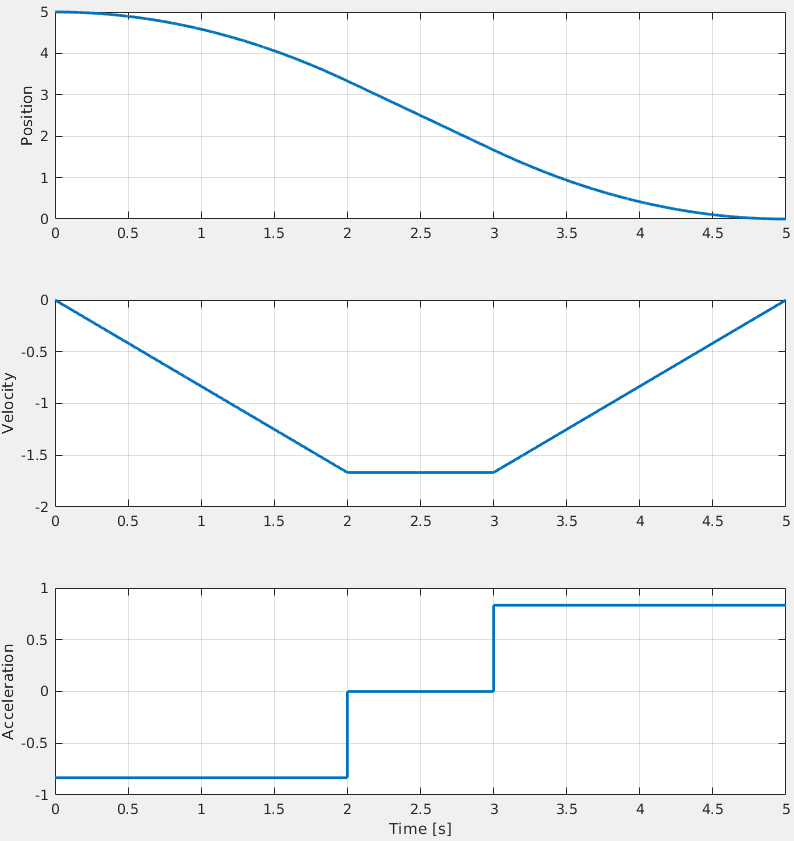
\includegraphics[keepaspectratio,width=\textwidth]{trap_2}
\caption{$t_c=2s, q_i>q_f$}
\label{fig:trap_2}
\end{minipage}
\begin{minipage}{0.333\textwidth}
\centering
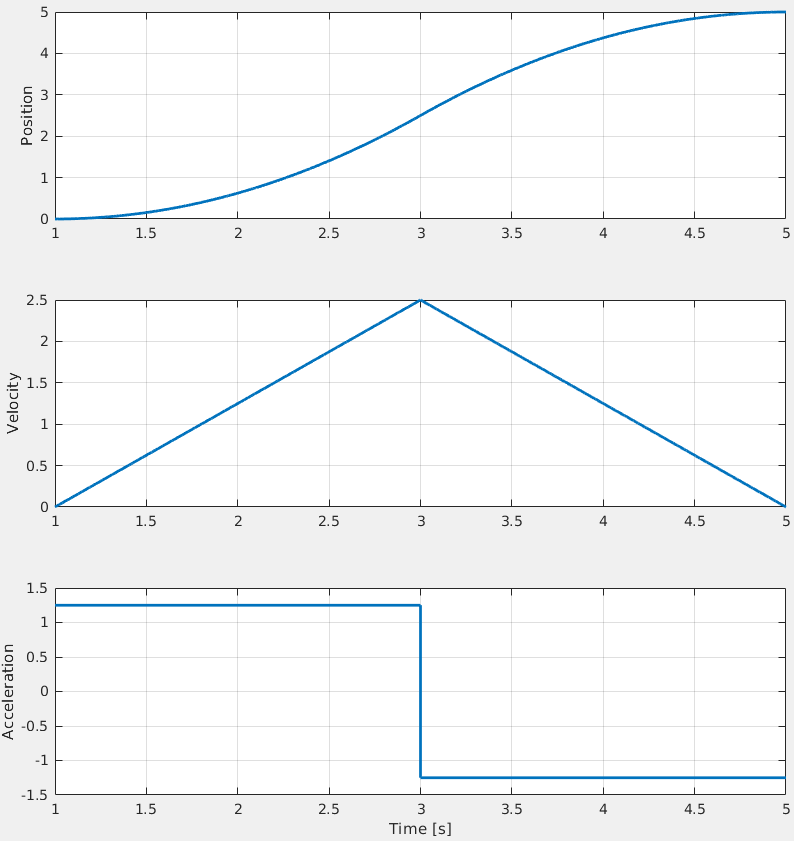
\includegraphics[keepaspectratio,width=\textwidth]{trap_3}
\caption{$t_c=2s, t_i\neq 0$}
\label{fig:trap_3}
\end{minipage}
\end{figure}

\begin{figure}
\begin{minipage}{0.5\textwidth}
\centering
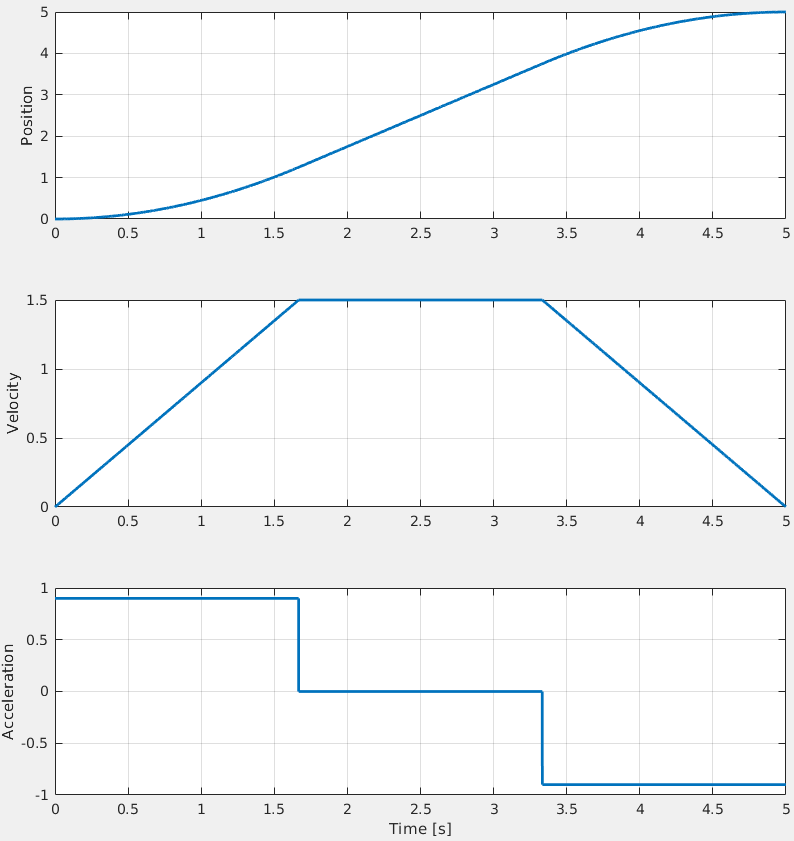
\includegraphics[keepaspectratio,width=\textwidth]{trap_5}
\caption{$v_c=1.5$}
\label{fig:trap_5}
\end{minipage}
\begin{minipage}{0.5\textwidth}
\centering
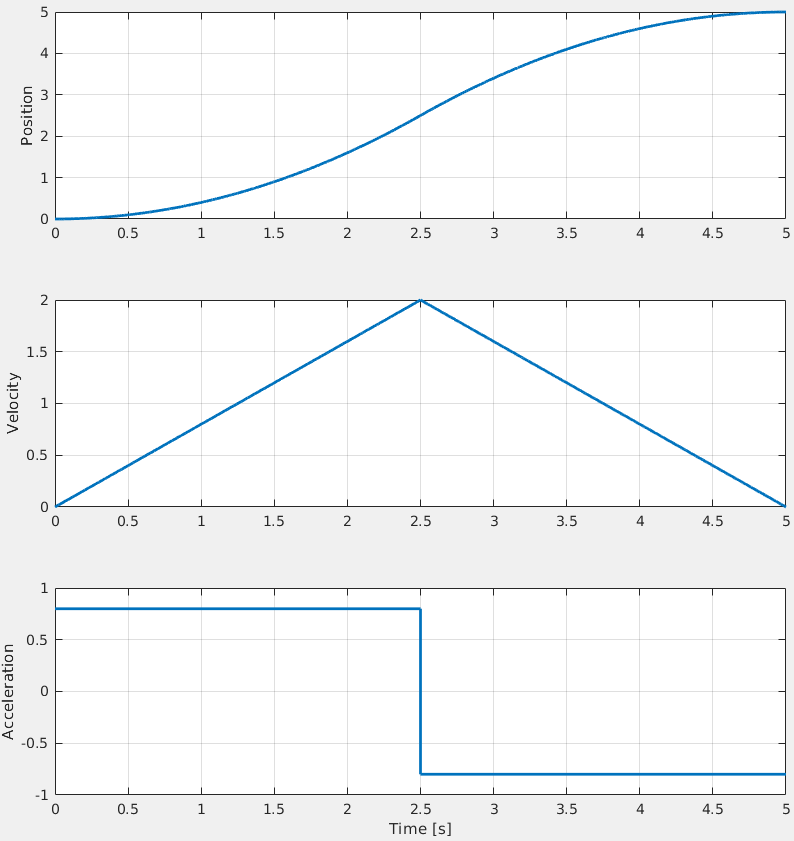
\includegraphics[keepaspectratio,width=\textwidth]{trap_4}
\caption{$v_c=v_{c,lim}=2$}
\label{fig:trap_4}
\end{minipage}
\end{figure}

\begin{figure}
\begin{minipage}{0.5\textwidth}
\centering
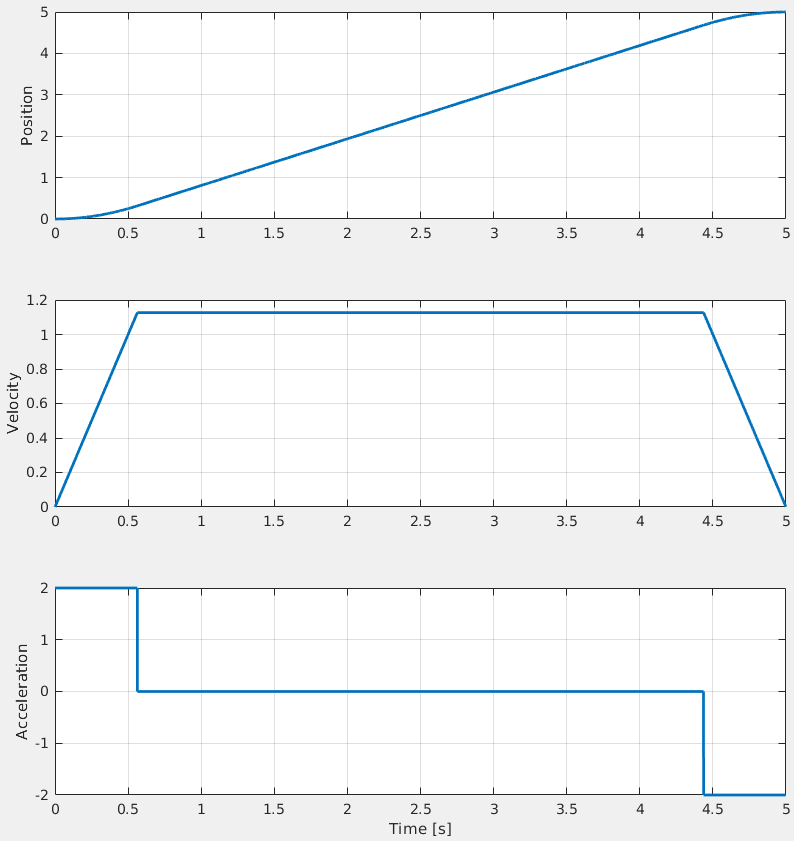
\includegraphics[keepaspectratio,width=\textwidth]{trap_6}
\caption{$a_c=2$}
\label{fig:trap_6}
\end{minipage}
\begin{minipage}{0.5\textwidth}
\centering
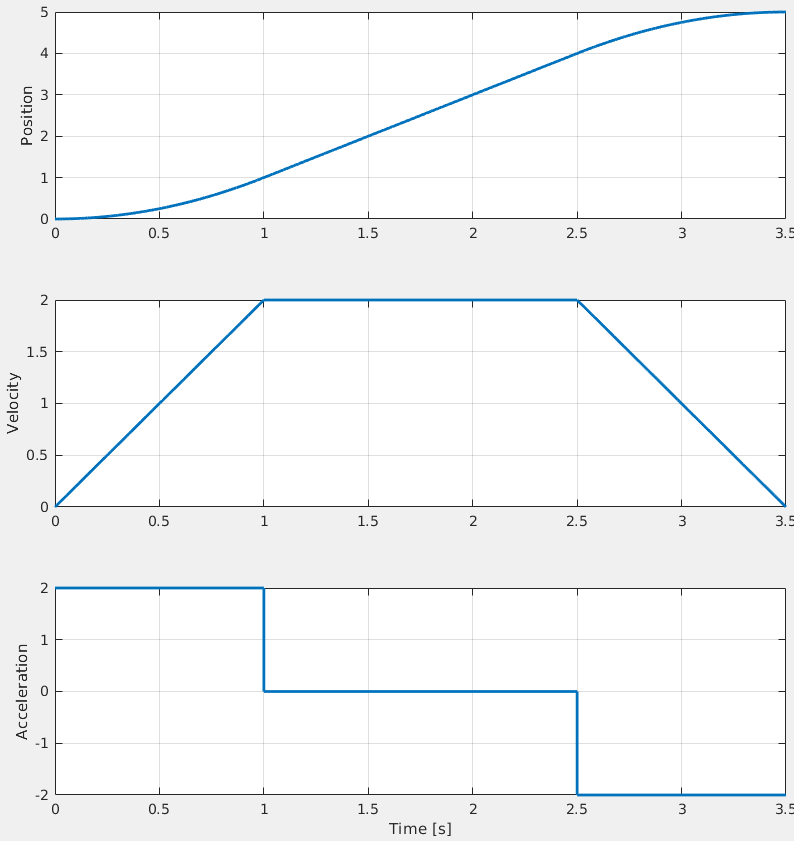
\includegraphics[keepaspectratio,width=\textwidth]{trap_7}
\caption{$a_c,v_c=2$}
\label{fig:trap_7}
\end{minipage}
\end{figure}

\begin{figure}
\begin{minipage}{0.5\textwidth}
\centering
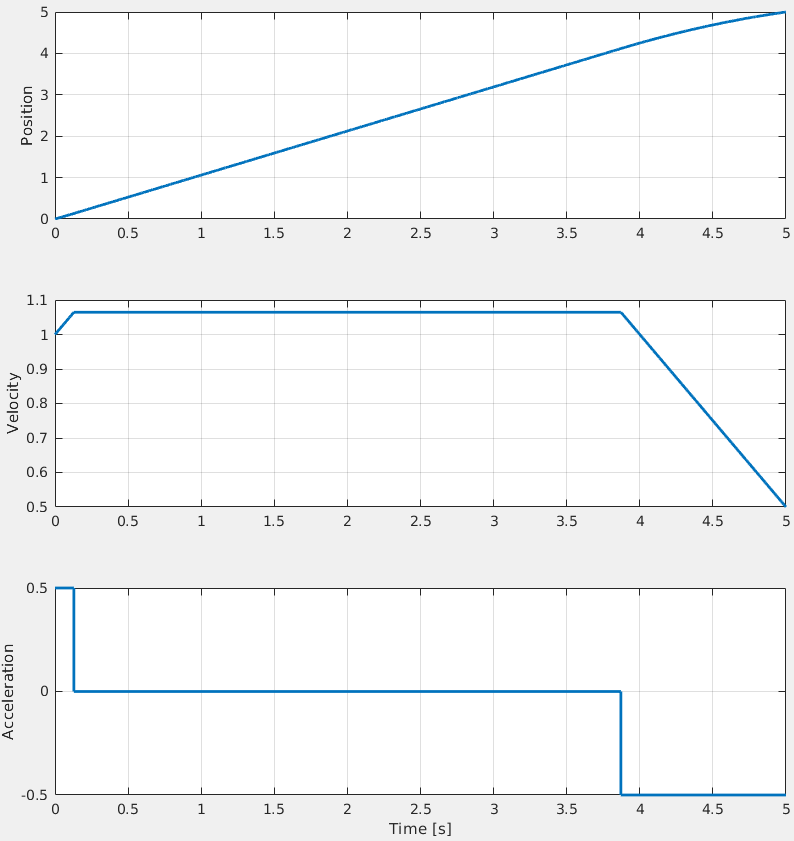
\includegraphics[keepaspectratio,width=\textwidth]{trap_8}
\caption{$\dot q_i=1,\dot q_f=0.5,\ddot q_{max}=0.5$}
\label{fig:trap_8}
\end{minipage}
\begin{minipage}{0.5\textwidth}
\centering
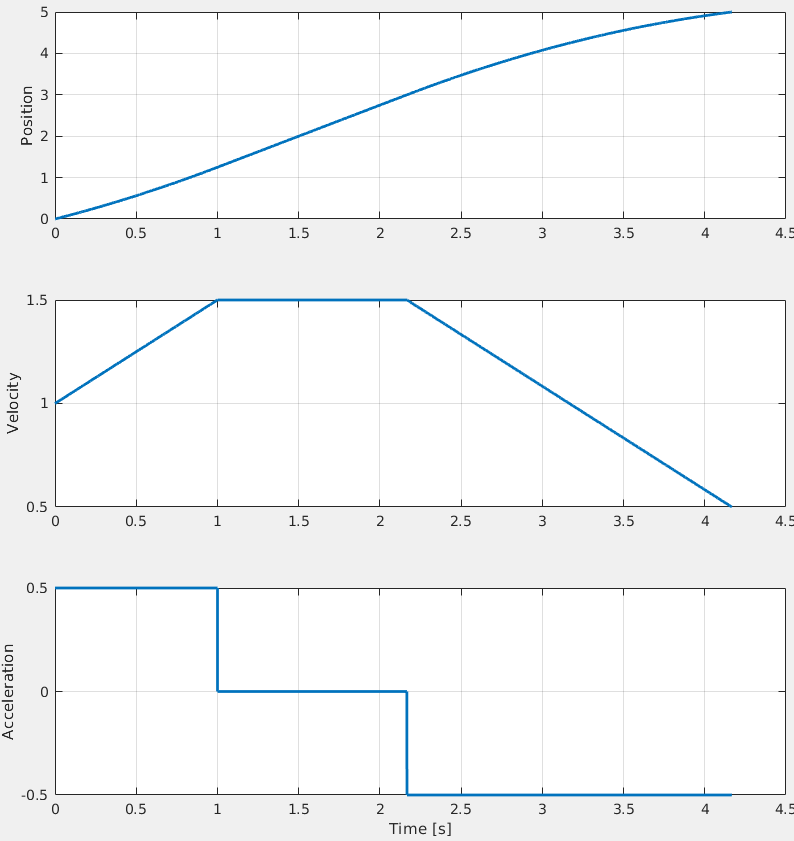
\includegraphics[keepaspectratio,width=\textwidth]{trap_9}
\caption{$\dot q_i=1,\dot q_f=0.5,\dot q_{max}=1.5,\ddot q_{max}=0.5$}
\label{fig:trap_9}
\end{minipage}
\end{figure}

To generate a multipoint trajectory we simply repeat the computation for each consecutive point pair. To improve the resulting velocity and acceleration profiles we can apply an heuristic to assign velocities to each waypoint, so that a less jagged profile is obtained:

\begin{align*}
\dot q(t_i)&=\dot q_i\\
\dot q(t_k)&=\begin{cases}
0 & \text{if }sign(\Delta Q_k)\neq sign(\Delta Q_{k+1})\\
sign(\Delta Q_k)\dot q_{max}& \text{if }sign(\Delta Q_k)= sign(\Delta Q_{k+1})\\
\end{cases}\\
\dot q(t_f)&=\dot q_f
\end{align*}

\begin{figure}
\begin{minipage}{0.5\textwidth}
\centering
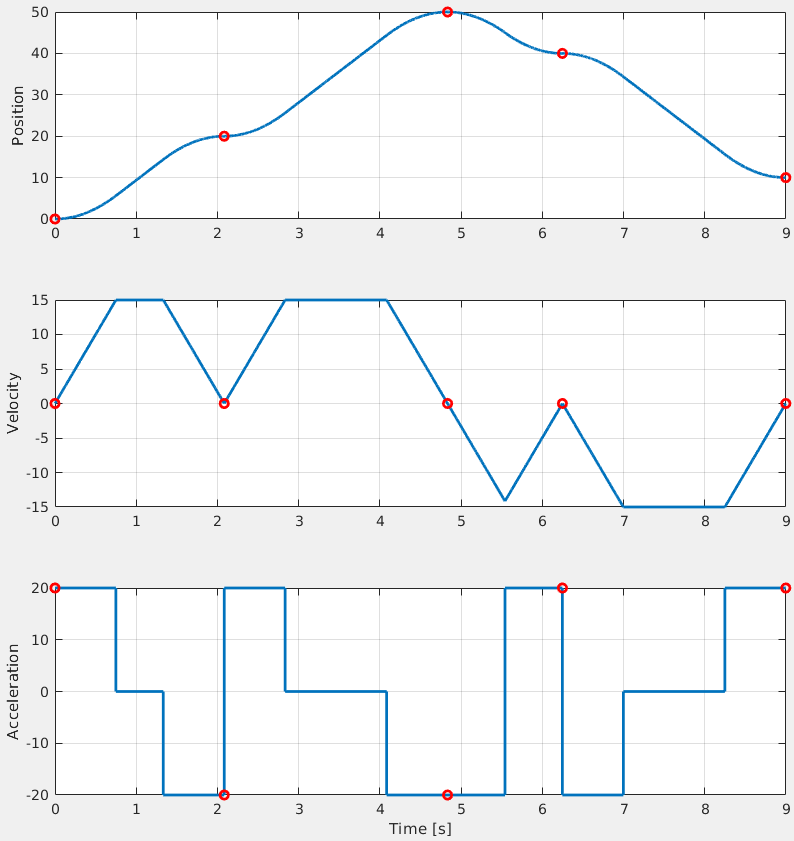
\includegraphics[keepaspectratio,width=\textwidth]{trap_10}
\caption{Multipoint trajectory without velocity heuristic}
\label{fig:trap_10}
\end{minipage}
\begin{minipage}{0.5\textwidth}
\centering
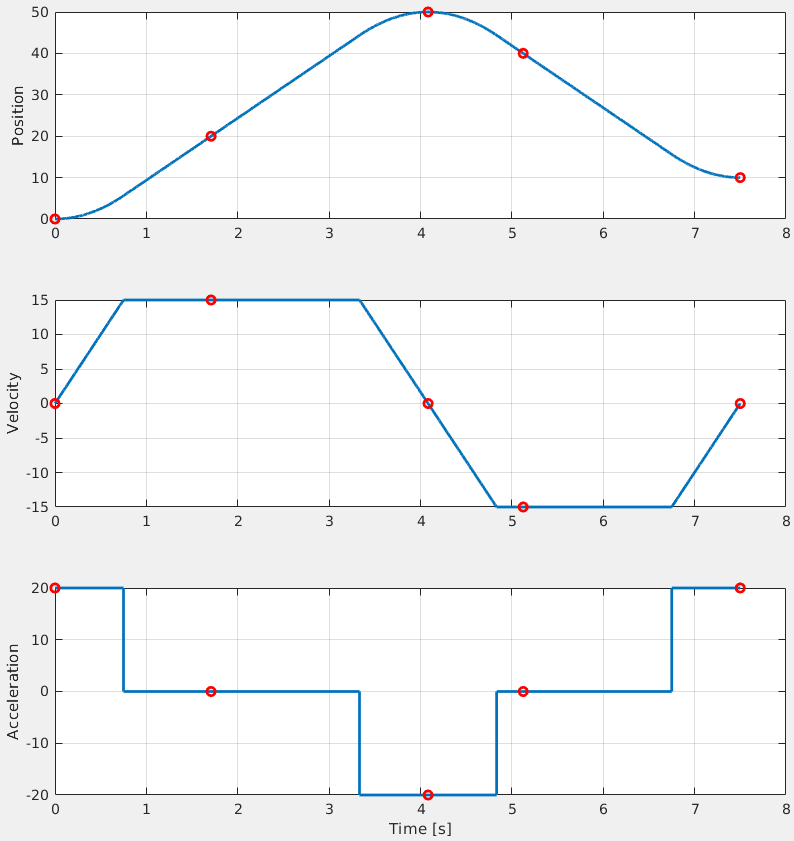
\includegraphics[keepaspectratio,width=\textwidth]{trap_11}
\caption{Multipoint trajectory with velocity heuristic}
\label{fig:trap_11}
\end{minipage}
\end{figure}